\documentclass[border=5mm]{standalone}
\usepackage{pgfplots}
\pgfplotsset{compat=1.18}

\begin{document}
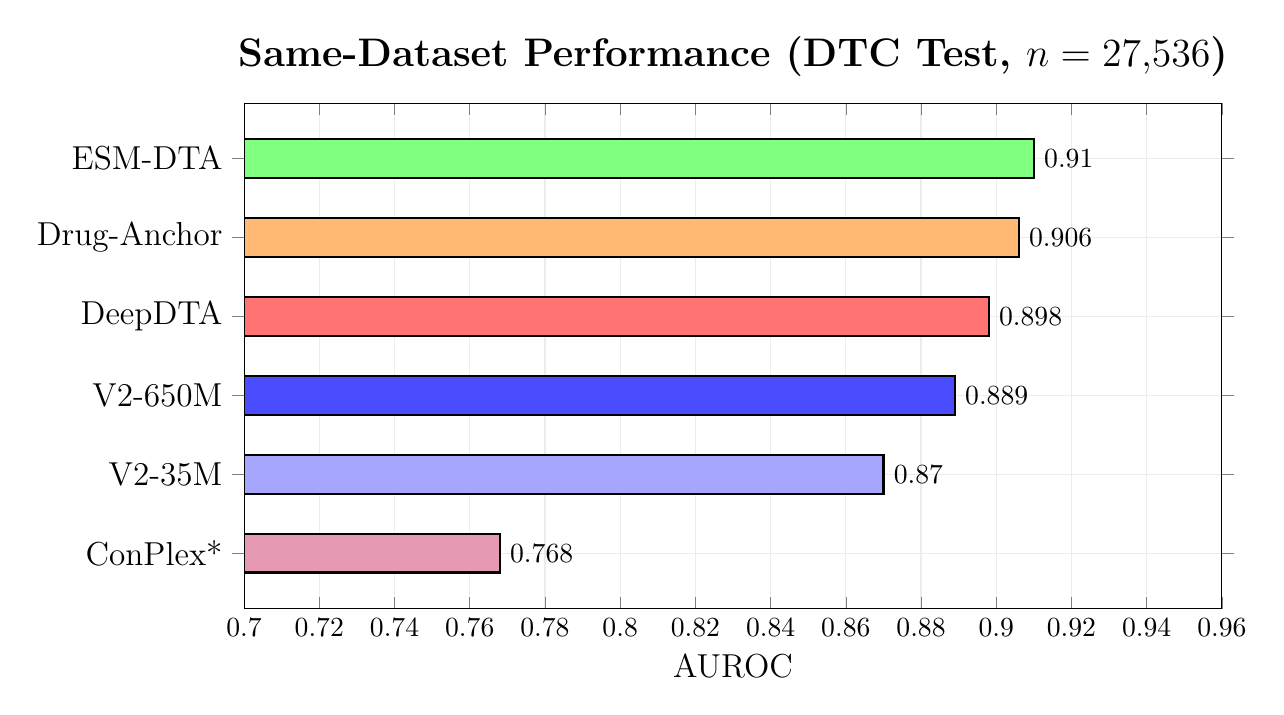
\begin{tikzpicture}
\begin{axis}[
    xbar,
    bar width=14pt,
    width=14cm,
    height=8cm,
    xlabel={AUROC},
    xlabel style={font=\large},
    ytick={0,1,2,3,4,5},
    yticklabels={ConPlex*, V2-35M, V2-650M, DeepDTA, Drug-Anchor, ESM-DTA},
    y tick label style={font=\large},
    ymin=-0.7, ymax=5.7,
    xmin=0.7, xmax=0.96,
    title={\textbf{Same-Dataset Performance (DTC Test, $n=27{,}536$)}},
    title style={font=\Large},
    nodes near coords,
    nodes near coords style={font=\normalsize, anchor=west, /pgf/number format/fixed, /pgf/number format/precision=3},
    grid=major,
    grid style={gray!15},
    xmajorgrids=true,
    every axis plot/.append style={thick},
]

\addplot[fill=purple!40, bar shift=0pt, forget plot] coordinates {(0.768, 0)};
\addplot[fill=blue!35, bar shift=0pt, forget plot] coordinates {(0.870, 1)};
\addplot[fill=blue!70, bar shift=0pt, forget plot] coordinates {(0.889, 2)};
\addplot[fill=red!55, bar shift=0pt, forget plot] coordinates {(0.898, 3)};
\addplot[fill=orange!55, bar shift=0pt, forget plot] coordinates {(0.906, 4)};
\addplot[fill=green!50, bar shift=0pt] coordinates {(0.910, 5)};

\end{axis}
\end{tikzpicture}
\end{document}
